\documentclass[14pt,a4paper]{book}
\usepackage[spanish,es-nodecimaldot]{babel}	% Utilizar español
\usepackage[utf8]{inputenc}					% Caracteres UTF-8
\usepackage{graphicx}						% Imagenes
\usepackage[hidelinks]{hyperref}			% Poner enlaces sin marcarlos en rojo
\usepackage{fancyhdr}						% Modificar encabezados y pies de pagina
\usepackage{float}							% Insertar figuras
\usepackage[textwidth=390pt]{geometry}		% Anchura de la pagina
\usepackage[nottoc]{tocbibind}				% Referencias (no incluir num pagina indice en Indice)
\usepackage{enumitem}						% Permitir enumerate con distintos simbolos
\usepackage[T1]{fontenc}					% Usar textsc en sections
\usepackage{amsmath}						% Símbolos matemáticos

\usepackage[table,xcdraw]{xcolor}
\setlength\headheight{26pt} 
\pagestyle{fancy}
\rhead{}

% Comandos para poner el nombre de la asignatura
\newcommand{\asignatura}{Metaheurística}
\newcommand{\autor}{Carlos Nuñez Molina \\ Ignacio Vellido Expósito}
\newcommand{\titulo}{SynVic}
\newcommand{\subtitulo}{Propuesta}

\begin{document}
    \pagenumbering{gobble}
    
% ==============================================================================
% Pagina de titulo
\begin{titlepage}
    \begin{minipage}{\textwidth}
        \centering

        
\includegraphics[scale=0.5]{images/ugr.png}\\

        \textsc{\Large \asignatura{}\\[0.2cm]}
        \textsc{GRADO EN INGENIERÍA INFORMÁTICA}\\[1cm]

        \noindent\rule[-1ex]{\textwidth}{1pt}\\[1.5ex]
        \textsc{{\Huge \titulo\\[0.5ex]}}
        \textsc{{\Large \subtitulo\\}}
        \noindent\rule[-1ex]{\textwidth}{2pt}\\[2.5ex]

        \end{minipage}

        \vspace{0.3cm}

        \begin{minipage}{\textwidth}

        \centering

        \textbf{Autores}\\ {\autor{}}\\[1.5ex]
        \vspace{0.2cm}

        
\includegraphics[scale=0.3]{images/etsiit.jpeg}

        \vspace{0.7cm}
        \textsc{Escuela Técnica Superior de Ingenierías Informática y de Telecomunicación}\\
        \vspace{1cm}
        \textsc{Curso 2019-2020}
    \end{minipage}
\end{titlepage}

% ==============================================================================
% ==============================================================================

    % ==============================================================================

    \chapter{Descripción}

SynVic es un juego free-to-play de acción MOBA y perspectiva isométrica. En él los jugadores se enfrentan en partidas cortas mediante batallas 2vs2, donde los jugadores deben formar equipo entre sí y explotar al máximo las sinergias entre sus personajes. Tras elegir un personaje, los jugadores entran en una sala con un mapa y un objetivo determinado (elegidos aleatoriamente de entre una gran variedad), una vez ahí deberán votar para formar equipo con el jugador que más le interese para alcanzar la victoria. Adicionalmente, los jugadores cuentan con la posibilidad de adaptar algunos detalles de las habilidades al mapa seleccionado y a las características de cada equipo. De esta manera se fomenta la cooperación en la preparación de la partida y la selección de sinergias.

\vspace{\baselineskip}

Nuestro público objetivo son jugadores de entre 15 y 30 años. A diferencia de la mayoría de MOBAs, queremos atraer tanto a jugadores casuales como fans del género MOBA. Esperamos que los casuals se sientan atraídos por las partidas cortas, frenéticas, y con una curva de dificultad inicialmente baja, pero creciente. A los más gamers pretendemos convencerlos con un ecosistema competitivo rico y variado que permita enfrentarse con gente de igual habilidad. También incluiremos un sistema de logros de personajes para que puedan demostrar su maestría con ellos. Todo esto junto a un soporte constante conseguirá un buen apoyo de la comunidad

\vspace{\baselineskip}

Las microtransacciones van a estar limitadas a aspectos estéticos del juego, siguiendo la fórmula de éxito de otros MOBAs y evitando el modelo de negocio pay-to-win que tanto odio genera entre los jugadores. Al eliminar la barrera de pago inicial impulsará en gran medida la llegada de nuevos jugadores.

\vspace{\baselineskip}

Centraremos el estilo artístico es un 2D simplificado (posiblemente las físicas sean en 3D), es decir, se pretende no sobrecargar con detalles/efectos a los jugadores y que el juego resulte claro e intuitivo a primera vista. La idea es tematizar los elementos con colores característicos que permitan identificarlos con facilidad. Así conseguimos que el arte sea funcional, aportando una utilidad para el jugador y no ser meramente decorativo.
    \chapter{Estudio de mercado}

El mercado orientado y en el cuál compite nuestro juego es el que rodea el género MOBA. Este está compuesto mayoritariamente de jugadores jóvenes, entre 12 y 35 años, atraídos por la experiencia multijugador con partidas competitivas y cooperativas. Generalmente este mercado prefiere sesiones de juego de corta duración (por debajo de la hora) pero con múltiples partidas.

\vspace{\baselineskip}

Este género se caracteriza principalmente por batallas multijugador con alto carácter competitivo, donde los jugadores eligen de entre una gran gama de personajes para luchar en partidas cortas sin ningún tipo de relación entre ellas. Por el estilo frenético y la necesidad de tener alta precisión hace que la plataforma principal a la que se orientan sea compatibles, aunque algunas compañías desarrollan una versión para consolas o móviles una vez adquieren éxito. Otra característica fundamental es el modelo de comercialización free-to-play, pues facilita la llegada de un gran número de aficionados.

\vspace{\baselineskip}

Los principales competidores que encontramos son: \textit{Battlerite}, \textit{League of Legends} y \textit{Heroes of the Storm}.

% ------------------------------------------------------------------------------
% ------------------------------------------------------------------------------

\section{Battlerite}

Lanzado en 2016 a manos de Stunlock Studios, sus autores lo definen como un \textit{arena de batallas}, un juego basado en la acción con batallas por equipos, en mapas de tamaño pequeño.
Con sistema monetario free-to-play, se lanzó inicialmente para Windows, y con un lanzamiento posterior en Xbox One.

\vspace{\baselineskip}

Se caracteriza por ser extremadamente frenético, con partidas cortas y emocionantes. Para ello renuncia a los sistemas de niveles y objetos centrándose púramente en la acción.

\vspace{\baselineskip}

Uno de sus problemas más destacados es la falta de variedad en los mapas. Al usar principalmente un modo de juego de deathmatch (matar un número predeterminado de veces al enemigo) la variedad de personajes no resulta suficiente para generar diferencias entre partidas. Por otro lado, no existe mucha sinergia entre las habilidades de estos personajes, por lo que no fomenta la cooperación en el equipo.

\vspace{\baselineskip}

Página web: https://arena.battlerite.com

\begin{figure}[H]
    \centering
    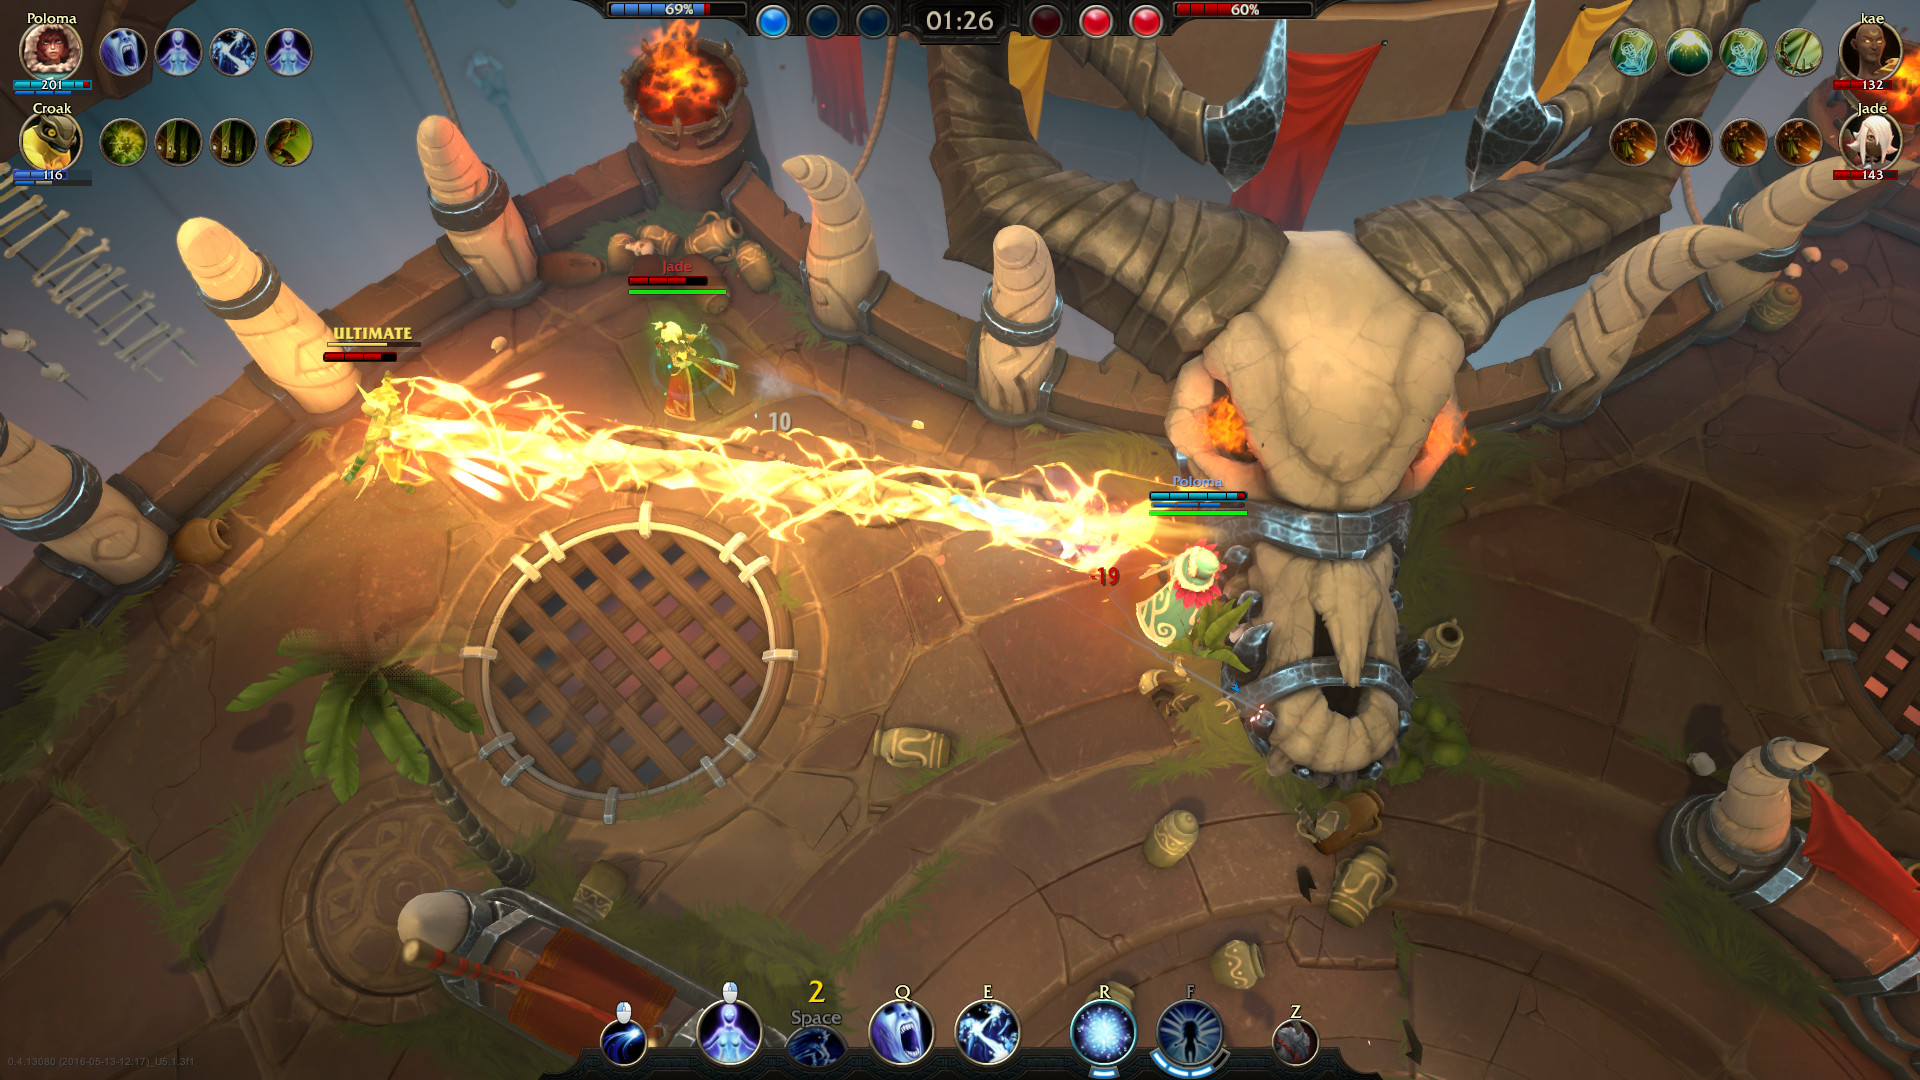
\includegraphics[width=0.95\columnwidth]{images/battlerite1.jpg}    
\end{figure}

\begin{figure}[H]
    \centering
    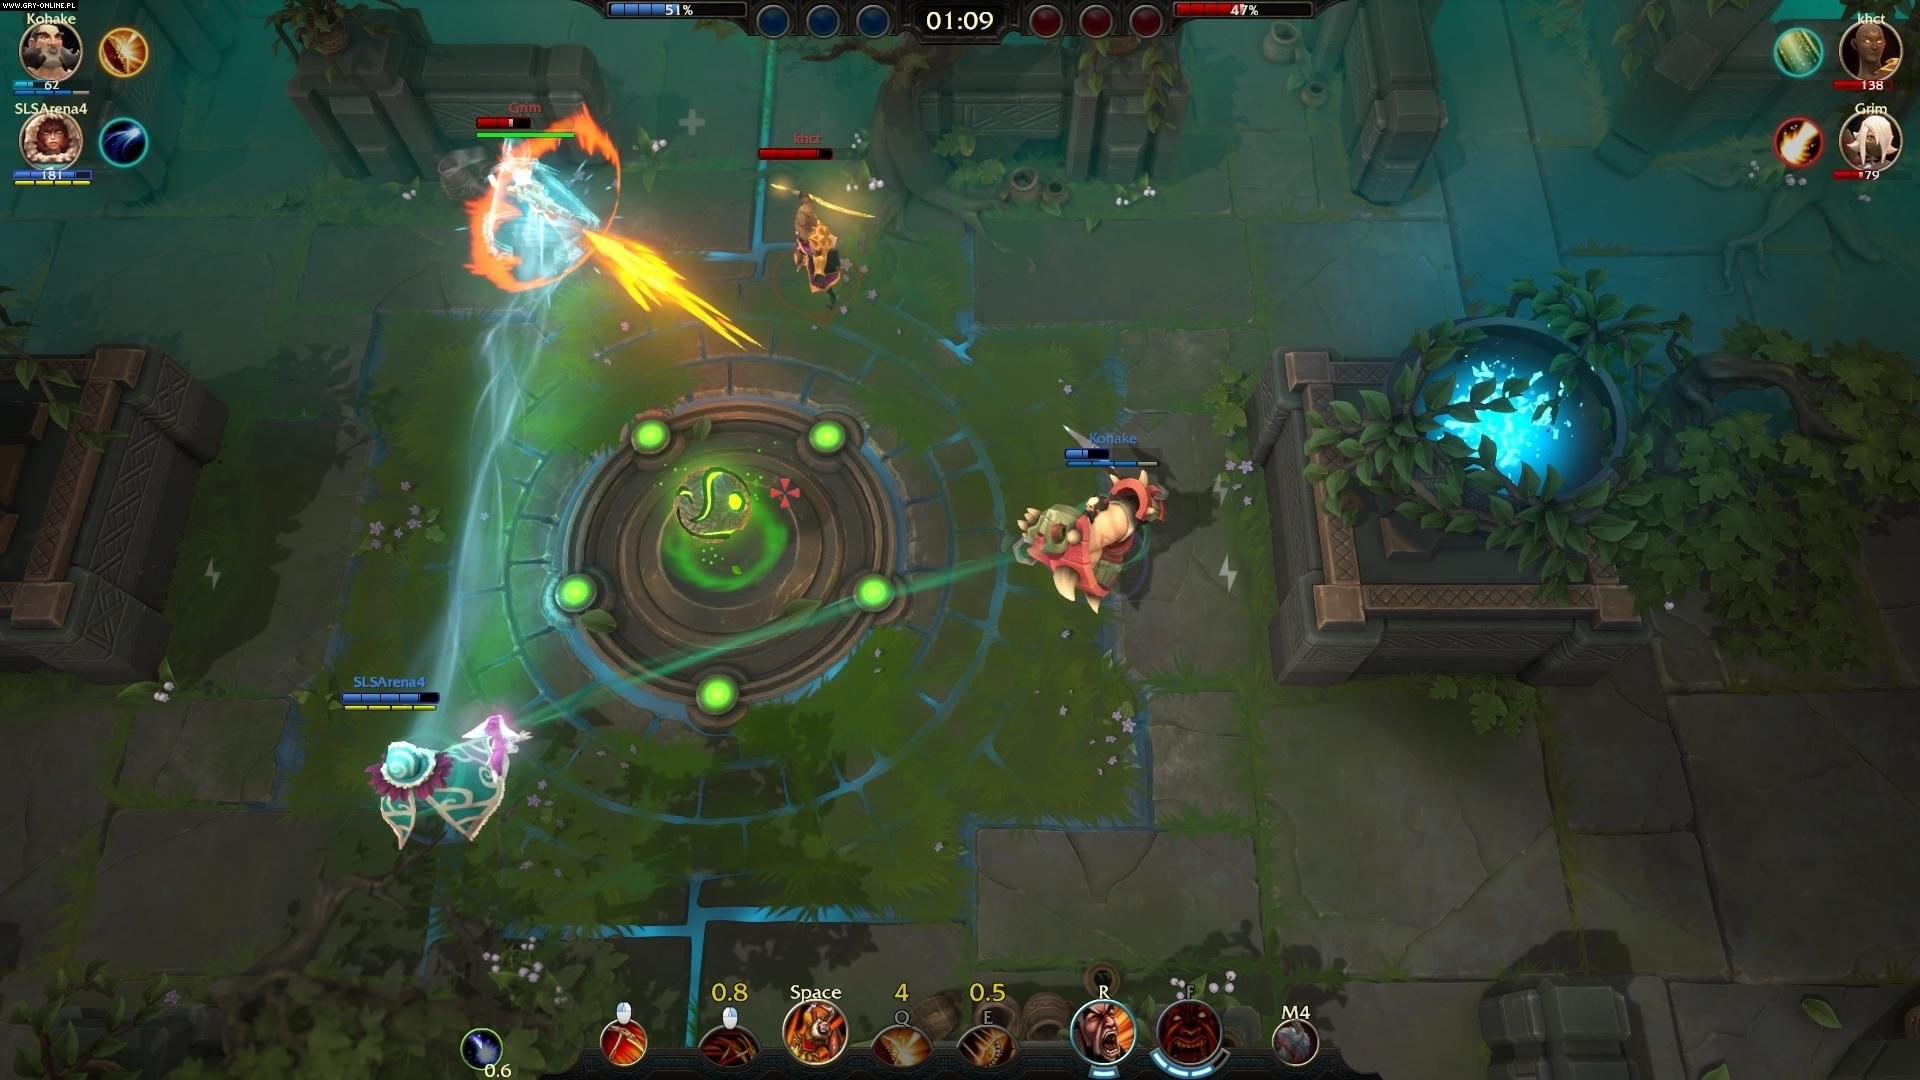
\includegraphics[width=0.95\columnwidth]{images/battlerite2.jpg}    
\end{figure}

% ------------------------------------------------------------------------------
% ------------------------------------------------------------------------------

\newpage

\section{League of Legends}

Desarrollado por Riot Games en 2009 para Windows, League of Legends continua el género MOBA creado por DOTA, consiguiendo impacto a nivel mundial.
Sigue la metodología free-to-play con micropagos cosméticos típica, que con el paso del tiempo se ha ido diversificando más allá de los aspectos de los personajes.

\vspace{\baselineskip}

Sus puntos más fuertes son los siguientes:

\begin{itemize}
    \item Mantiene soporte y actualizaciones constantes, centradas en mayor medida en mejorar la experiencia de los jugadores.
    \item Creatividad y diversidad en el diseño de personajes. Partiendo de un número inicial de 40 en 10 años han alcanzado casi los 150.
    \item Buena curva de dificultad, produciendo la sensación de que siempre se puede mejorar. Comparado con su gran competidor, DOTA2, resulta más sencillo entender las mecánicas y estrategias que requiere el juego.
    \item Tras la actualización visual de 2014 el aspecto artístico del mapa mejoró drásticamente, consiguiendo un estilo limpio y claro.
    \item Fuertemente involucrado con los e-sports, empujando la marca más allá del juego.
\end{itemize}

Por contra, el viaje de LoL a lo largo de los años ha estado cargado de fallos, entre ellos:

\begin{itemize}
    \item Numerosos errores técnicos: fallos de balanceo, infraestructura de red, cliente\dots. El excesivo número de lanzamientos de personajes, y la necesidad de que estos sean útiles y llamativos (para fomentar la compra) es buena causa de ello.
    \item Poco control sobre la comunidad, lo que genera mala experiencia con temas de abuso verbal, trolling\dots
    \item Progresión no satisfactoria, más allá de mejorar como jugador existen pocas recompensas por jugar.
    \item En ocasiones las partidas resultan largas y pesadas, rondando los 40 minutos y alcanzando la hora en caso extremos.
\end{itemize}

Página web: http://leagueoflegends.com/

\begin{figure}[H]
    \centering
    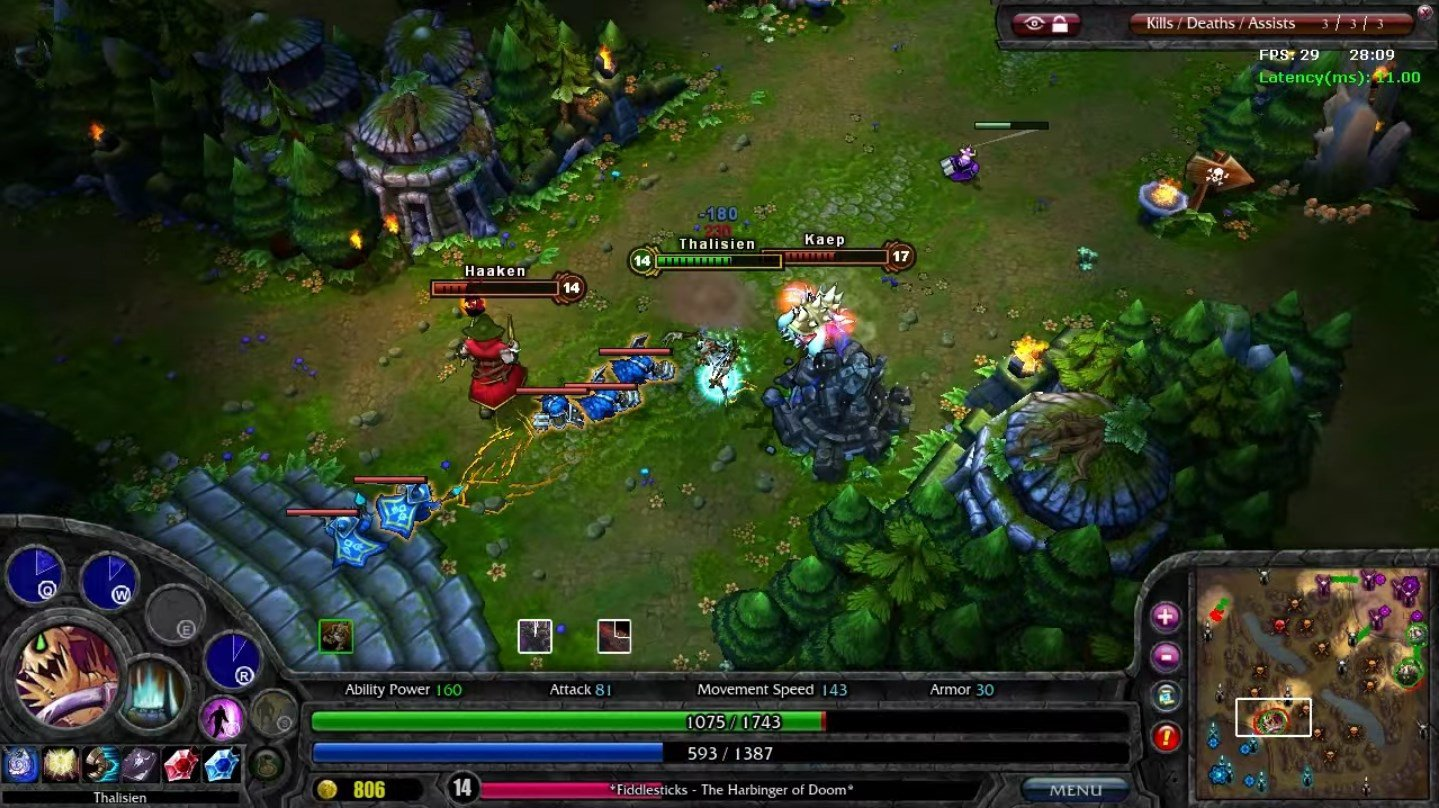
\includegraphics[width=0.95\columnwidth]{images/lol1.jpg}    
    \caption{League of Legends en sus primeros años}
\end{figure}

\begin{figure}[H]
    \centering
    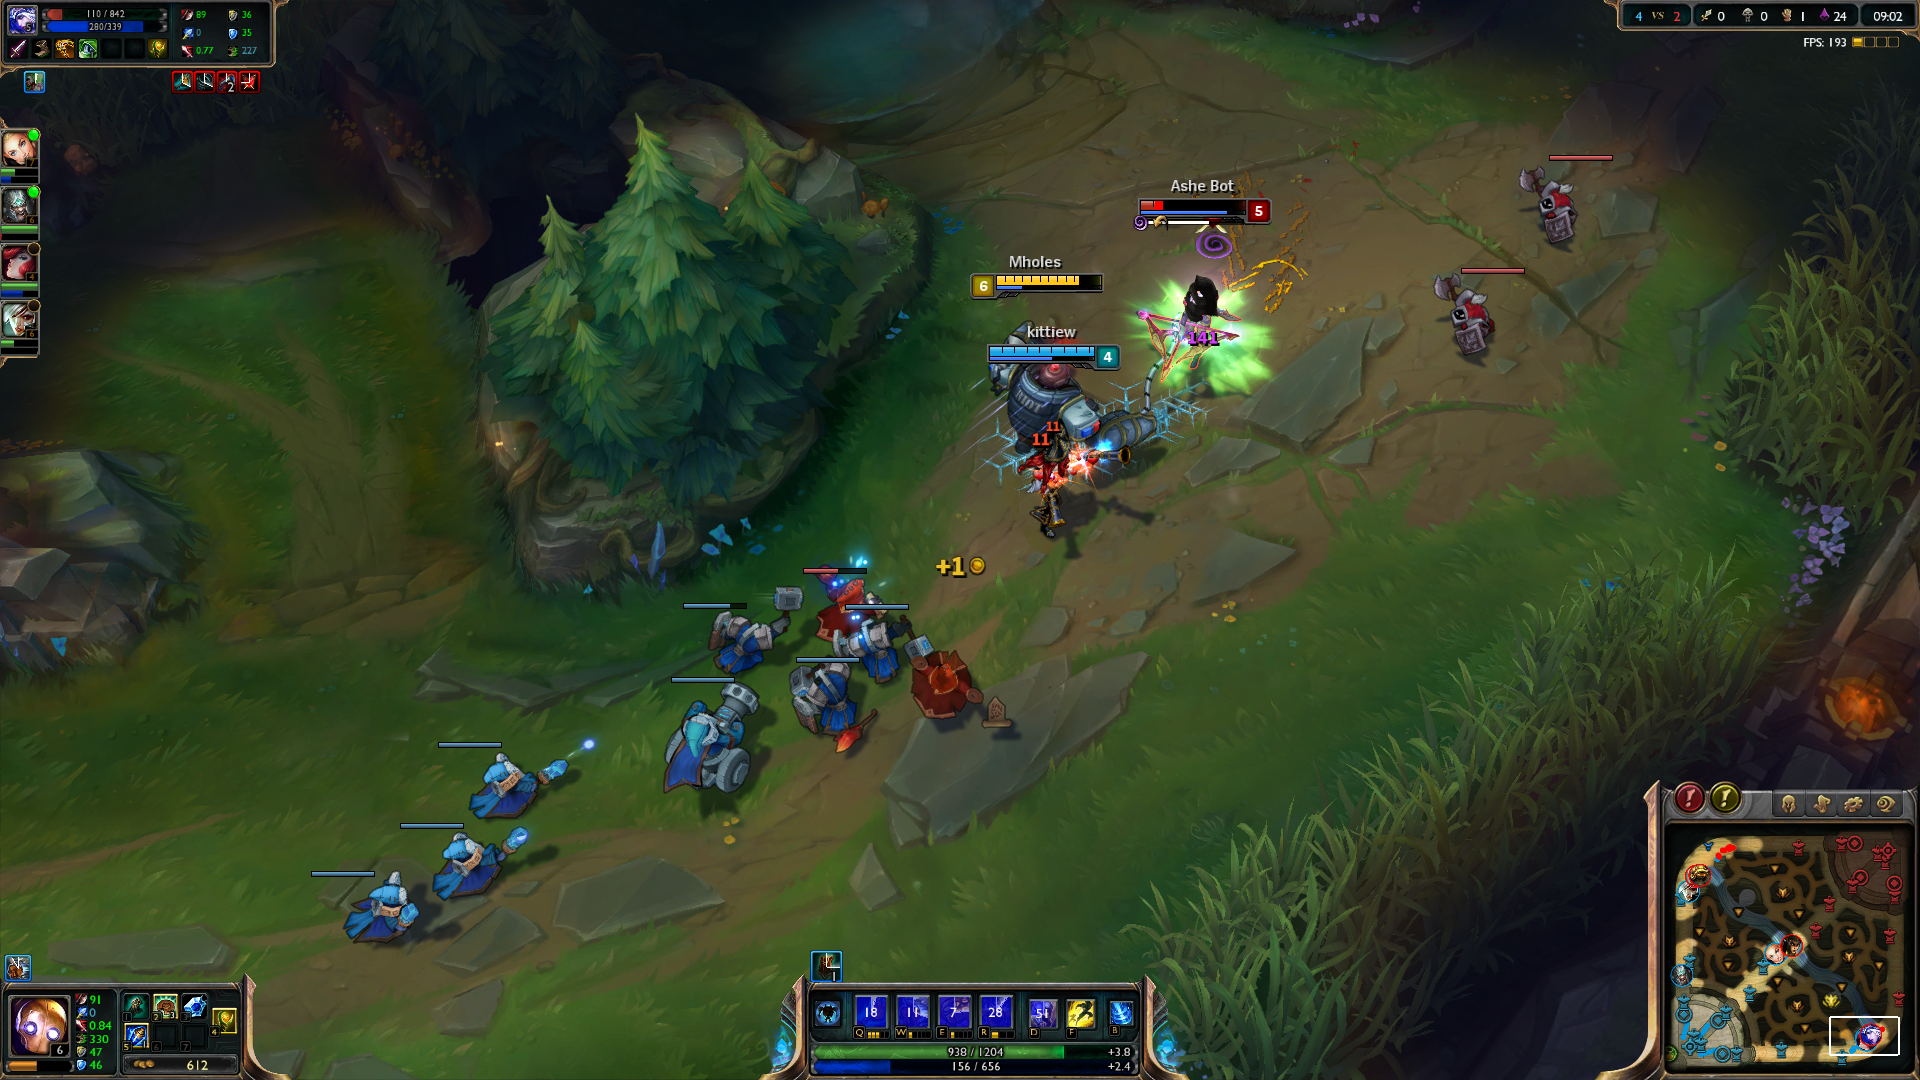
\includegraphics[width=0.95\columnwidth]{images/lol2.png}
    \caption{Tras la actualización visual}
\end{figure}

% ------------------------------------------------------------------------------
% ------------------------------------------------------------------------------

\newpage

\section{Heroes of the Storm}

Desarrollado por Blizzard en 2015, HoTS es otra gran competidor dentro del género MOBA, aunque actualmente ha ido perdiendo el interés de la comunidad. También lanzado para compatibles (Windows y MacOS) con el modelo free-to-play y micropagos cosméticos.

\vspace{\baselineskip}

El gran atractivo de HotS fue un buen uso de la marca Blizzard atrayendo tanto a jugadores del género MOBA como a fans de sus marcas Warcraft, Starcraft y Diablo. Teniendo las siguientes características positivas:

\begin{itemize}
    \item Gran variedad de mapas con diversos objetivos entre ellos.
    \item Elimina sistema de puntuaciones individuales. Las bajas y los objetivos las adquiere el equipo en sí. Esto sacrifica parte de la estrategia monetaria de juegos como LoL y DOTA pero evita enfrentar a los jugadores con sus estadísticas personales.
\end{itemize}

Estas puntos no han sido suficientes para hacer triunfar el juego a gran escala, y es que cuenta con fallos como:

\begin{itemize}
    \item Su mayor problema fue una llegada tardía al género incluyendo pocas novedades, y pocas de ellas diferenciadoras de la competencia.
    \item Visualmente confuso, cargado de detalles. Los colores no realzan ni diferencian los objetos entre sí. El HUD tiene un diseño simple, pero partes como el minimapa tienen una selección de colores no apropiada (se confunden con ciertas zonas del escenario).
\end{itemize}

Página web: https://heroesofthestorm.com/

\begin{figure}[H]
    \centering
    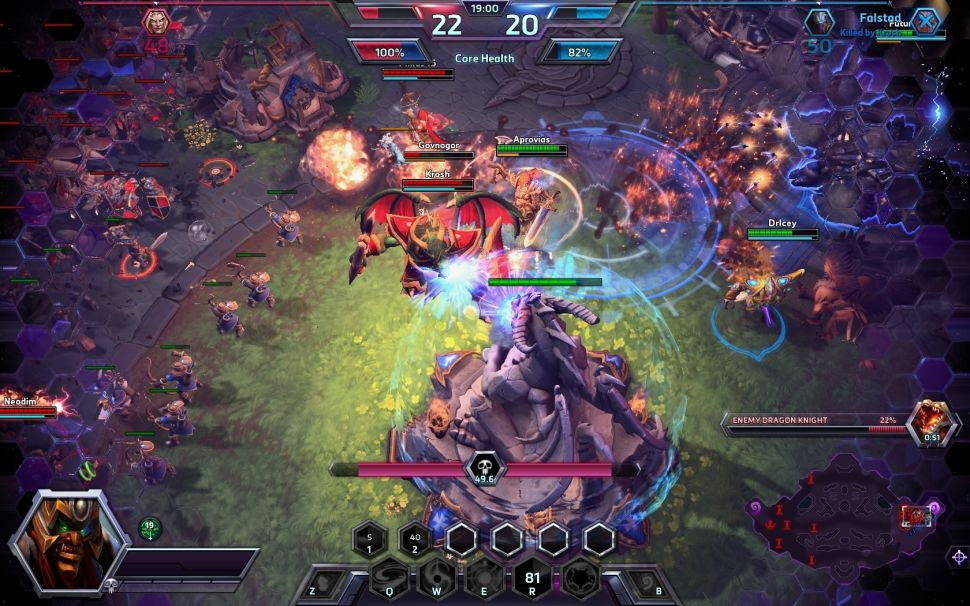
\includegraphics[width=0.95\columnwidth]{images/hots1.jpg}    
\end{figure}

\begin{figure}[H]
    \centering
    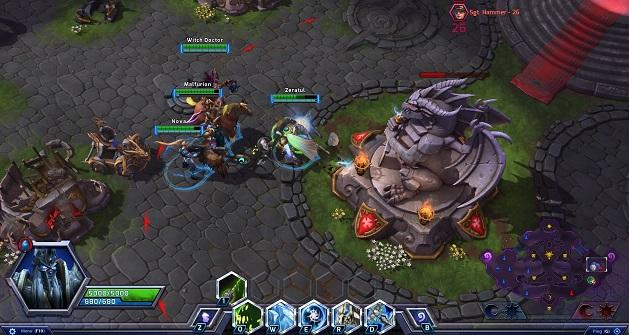
\includegraphics[width=0.95\columnwidth]{images/hots2.jpg}    
\end{figure}

    \setlength{\parskip}{1em}
    
    % ==============================================================================
\end{document}


\end{document}